\documentclass[10pt,a4paper]{article}
\usepackage[latin1]{inputenc}
\usepackage{amsmath}
\usepackage{amsfonts}
\usepackage{amssymb}
\usepackage{fullpage}
\usepackage{graphicx}

\begin{document}
\title{J.D. Jackson Problem 9.16}
\author{Josh Orndorff \\ admin@joshorndorff.com}
\maketitle

\section{Power Radiated per Unit Solid Angle}
We'll start by writing a functional form for the current density at all points in space.  We know that the current in the rod is given by $I(z')=I_0\sin kz \hat{\mathbf{z}}$.  But we have to dress this up as $J(\mathbf{x})$.  Note that the wave number $k=\frac{2\pi}{d}$.

\begin{equation}
\mathbf{J}(\mathbf{x})=\delta(x)\delta(y)I(z')=I_0\sin kz [\Theta(z+d/2)-\Theta(z-d/2)]\hat{\mathbf{z}}
\end{equation}

Using Equation 9.8 from Jackson, we can find the vector potential
\begin{equation}
\mathbf{A}(\mathbf{x})=\frac{\mu_0}{4\pi}\frac{e^{ikr}}{r}\int_{All Space}\mathbf{J}(\mathbf{x'})e^{-ik\hat{\mathbf{n}}\cdot\mathbf{x'}} \mathrm{d}^3\mathbf{x'}
\end{equation}

In the geometry of our problem, $\hat{\mathbf{n}}\cdot\mathbf{x'} = z'\cos\theta$.
\begin{equation}
\mathbf{A}(\mathbf{x})=\frac{\mu_0}{4\pi}\frac{e^{ikr}}{r}\int_{-d/2}^{d/2}I_0\sin kz'e^{-ikz'\cos\theta}\hat{\mathbf{z}} \mathrm{d}z'
\end{equation}

Now we'll use Euler's formula to expand the integral.
\begin{equation}
\mathbf{A}(\mathbf{x})=\frac{\mu_0 I_0}{4\pi}\frac{e^{ikr}}{r}\int_{-d/2}^{d/2}\sin (kz') \cos(kz'\cos\theta)-i\sin (kz') \sin(kz'\cos\theta) \hat{\mathbf{z}} \mathrm{d}z'
\end{equation}

The first term in the integral is zero because the sine function is odd and the cosine function is even.
\begin{equation}
\mathbf{A}(\mathbf{x})=\frac{-i\mu_0 I_0}{4\pi}\frac{e^{ikr}}{r}\int_{-d/2}^{d/2}\sin (kz') \sin(kz'\cos\theta) \hat{\mathbf{z}} \mathrm{d}z'
\end{equation}

Using an obscure trig identity, $2 \sin s \sin t = \cos(s-t) - \cos(s+t)$, we can turn the product of sines into a difference of cosines which will be easier to integrate.

\begin{equation}
\mathbf{A}(\mathbf{x})=\frac{-i\mu_0 I_0}{4\pi}\frac{e^{ikr}}{r}\int_{-d/2}^{d/2}\frac{1}{2}\left[
\cos[kz'(1-\cos\theta)]-\cos[kz'(1+\cos\theta)]
\right] \mathrm{d}z'
\end{equation}

Finally we can perform the actual integration.
\begin{equation}
\mathbf{A}(\mathbf{x})=\frac{-i\mu_0 I_0}{8\pi k}\frac{e^{ikr}}{r}\hat{\mathbf{z}}\left[
\frac{sin[kz'(1-\cos\theta)]}{1-\cos\theta}-\frac{sin[kz'(1+\cos\theta)]}{1+\cos\theta}
\right]_{-d/2}^{d/2}
\end{equation}

Simplifying, and substituting $k=2\pi/d$ in the leading fraction,
\begin{equation}
\mathbf{A}(\mathbf{x})=\frac{-i\mu_0 I_0 d}{8 \pi^2}\frac{e^{ikr}}{r}\hat{\mathbf{z}}\left[
\frac{sin[\pi(1-\cos\theta)]}{1-\cos\theta}-\frac{sin[\pi(1+\cos\theta)]}{1+\cos\theta}
\right]
\end{equation}

Simplifying the terms in square brackets is a bit long, and is covered separately in appendix A. If you're interested in a less rigorous solution, proceed happily to the final form below.

After all that simplification, we obtain this form for the vector potential.
\begin{equation}
\mathbf{A}(\mathbf{x})=\frac{-i\mu_0 I_0 d}{4 \pi^2}\frac{e^{ikr}}{r}\frac{\sin(\pi\cos\theta}{\sin^2\theta}\hat{\mathbf{z}}
\end{equation}

Equation 9.16 in Jackson's text relates vector potential $\mathbf{A}$, and dipole moment, $\mathbf{p}$. We'll rearrange that equation to solve for $\mathbf{p}$.
\begin{equation}
\mathbf{p}=-\frac{r}{e^{ikr}}\frac{4\pi}{i\mu_0\omega}\mathbf{A}(\mathbf{x})
\end{equation}

Plugging in the vector potential that we found, we see that
\begin{equation}
\mathbf{p}=-\frac{r}{e^{ikr}}\frac{4\pi}{i\mu_0\omega}\left[\frac{-i\mu_0 I_0 d}{4 \pi^2}\frac{e^{ikr}}{r}\frac{\sin(\pi\cos\theta}{\sin^2\theta}\right]
\end{equation}

\begin{equation}
\mathbf{p}=\frac{I_0 d}{\pi\omega}\frac{\sin(\pi\cos\theta}{\sin^2\theta}\hat{\mathbf{z}}
\end{equation}

Finally, to get the power distribution, we can use Equation 9.23 from the text.
\begin{equation}
\frac{\mathrm{d}P}{\mathrm{d}\Omega}= \frac{c^2 Z_0}{32 \pi^2}k^4|\mathbf{p}|^2\sin^2\theta
\end{equation}

Plugging in our form for dipole moment,
\begin{equation}
\frac{\mathrm{d}P}{\mathrm{d}\Omega}= \frac{c^2 Z_0}{32 \pi^2}k^4\frac{\sin^2(\pi\cos\theta)}{\sin^4\theta}\sin^2\theta
\end{equation}

Remembering $k=\frac{\omega}{c}$ and $d=\frac{2\pi}{k}$, and cancelling the appropriate terms,
\begin{equation}
\frac{\mathrm{d}P}{\mathrm{d}\Omega}=\frac{Z_0I_0^2}{8\pi^2}\frac{\sin^2(\pi\cos\theta)}{\sin^2\theta}
\end{equation}


\begin{figure}[hbtp]
\caption{Altitudinal dependence of power in units of $\frac{Z_0I_0^2}{8\pi}$.}
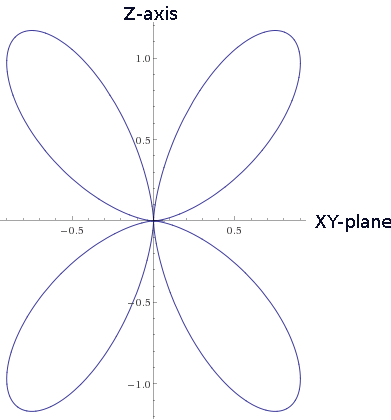
\includegraphics[scale=1]{Jackson9-16-plot.png}
\end{figure}


\section{Total Power Radiated}
The total power radiated is calculated by integrating over all solid angles.
\begin{equation}
P=\frac{Z_0I_0^2}{8\pi^2}\int_0^{2\pi}\int_0^\pi
\frac{\sin^2(\pi\cos\theta)}{\sin^2\theta}
\sin\theta\, \mathrm{d}\theta \, \mathrm{d}\phi
\end{equation}

The azimuthal integral is easy because the radiation pattern is azimuthally symmetric.
\begin{equation}
P=\frac{Z_0I_0^2}{4\pi}\int_0^\pi
\frac{\sin^2(\pi\cos\theta)}{\sin^2\theta}
(\sin\theta\, \mathrm{d}\theta)
\end{equation}

Evaluating the altitudinal integral will require a substitution, $x=\cos\theta$ such that $\mathrm{d}x=-\sin\theta\,\mathrm{d}\theta$.
\begin{equation}
P=-\frac{Z_0I_0^2}{4\pi}\int_1^{-1}
\frac{\sin^2(\pi x)}{1-x^2}
\, \mathrm{d}x
\end{equation}

The closed form of the integral in question is not particularly insightful, but the result is.
\begin{equation}
P\approx\frac{Z_0I_0^2}{4\pi}(1.57542)
\end{equation}

To find the radiation resistance, we recall that $P=\frac{1}{2}I_0^2R$ (is this in Jackson or something??).
\begin{equation}
R=\frac{2P}{I_0^2}=\frac{Z_0}{2\pi}(1.57542)=.2507\,Z_0
\end{equation}


\appendix
\section{Simplifying the Vector Potential Integral}
We'll start with this expression, and explain the simplifications line by line.
\begin{equation}
\frac{sin[\pi z'(1-\cos\theta)]}{1-\cos\theta}-\frac{sin[\pi z'(1+\cos\theta)]}{1+\cos\theta}
\end{equation}

I'll first distribute the $\pi$ inside the argument of the numerator.
\begin{equation}
\frac{sin[\pi-\pi\cos\theta]}{1-\cos\theta}-\frac{sin[\pi+\pi\cos\theta)]}{1+\cos\theta}
\end{equation}

The next step is to get a common denominator.
\begin{equation}
\frac{
\sin(\pi(1-\cos\theta))(1+\cos\theta)-\sin(\pi(1+\cos\theta))(1-\cos\theta)
}{1-\cos^2\theta}
\end{equation}


Now we can use the angle difference formula, $\sin(s-t) = \sin s \cos t - \cos s \sin t$, to expand each term in the numerator. I'll also multiply the resulting binomials in this step.
\begin{multline}
\frac{1}{sin^2\theta}[
\sin\pi\cos(\pi\cos\theta)
-\cos\pi\sin(\pi\cos\theta)
+\sin\pi\cos(\pi\cos\theta)\cos\theta
-\cos\pi\sin(\pi\cos\theta)\cos\theta \\
-\sin\pi\cos(\pi\cos\theta)
-\cos\pi\sin(\pi\cos\theta)
+\sin\pi\cos(\pi\cos\theta)\cos\theta
+\cos\pi\sin(\pi\cos\theta)\cos\theta
]
\end{multline}

The first, third, fifth, and seventh terms above contain $\sin\pi$ and are consequently zero.  The remaining terms simplify slightly because they contain $\cos\pi=-1$.
\begin{equation}
\frac{1}{sin^2\theta}[
\sin(\pi\cos\theta)
+\sin(\pi\cos\theta)\cos\theta
+\sin(\pi\cos\theta)
-\sin(\pi\cos\theta)\cos\theta
]
\end{equation}

The second and fourth terms above cancel, while the first and third terms combine to give the final simplified form.
\begin{equation}
\frac{2}{\sin^2\theta}\sin(\pi\cos\theta)
\end{equation}

\section{The Two Wavelength Problem}
Let's investigate how the problem would be different if two complete waves stood on the antenna instead of just one.
\end{document}